\graphicspath{{./images/molecules/orbitals/hbbnc/}}
\begin{figure}[h!]
	\centering
%\begin{minipage}{\textwidth}\centering
%\mybox{
%\begin{tabular}{lrccc}
%\multicolumn{2}{c}{\textbf{Tetra-Pyrene}} & Model & HOMO & LUMO\\
%\multicolumn{2}{c}{\textbf{}}
%&\multirow{3}{*}{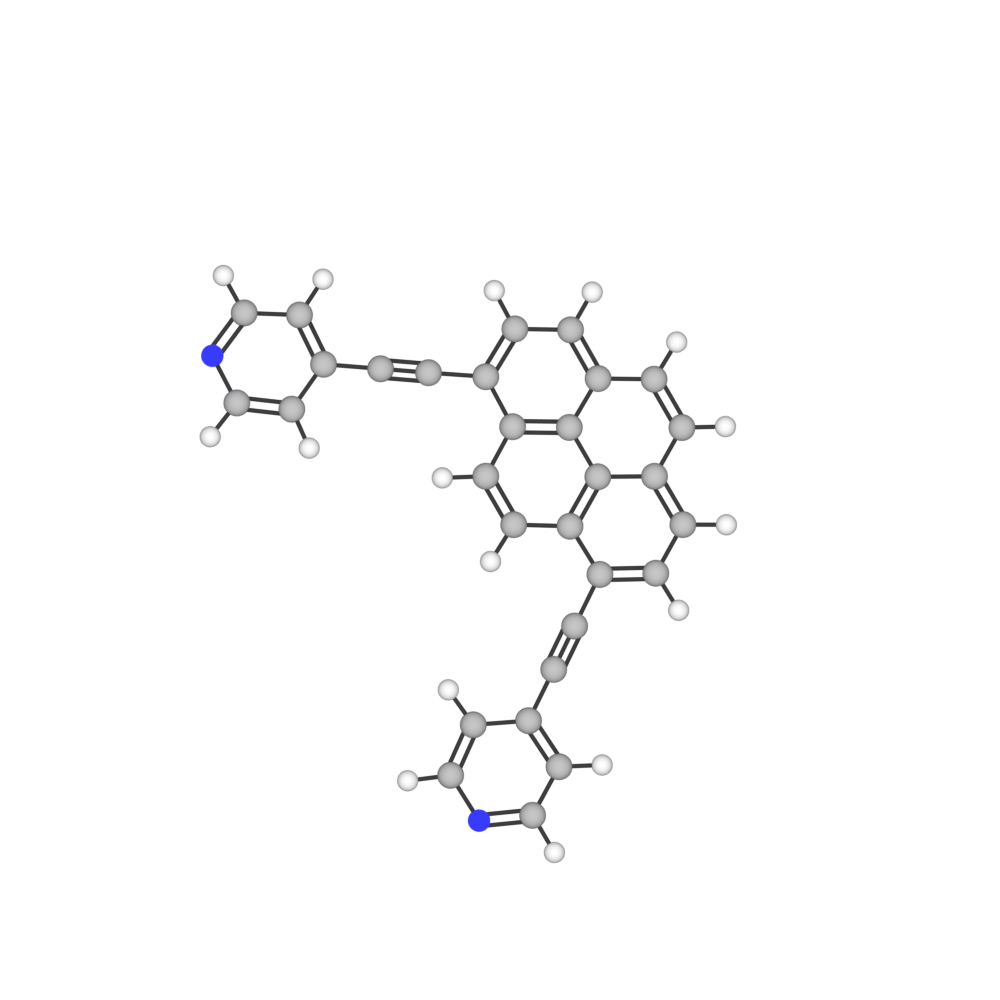
\includegraphics[width=2.7cm]{model}}
%&\multirow{3}{*}{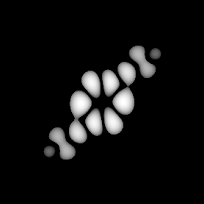
\includegraphics[width=2.7cm]{homo}}
%&\multirow{3}{*}{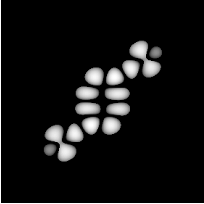
\includegraphics[width=2.7cm]{lumo}}\\
%&&&& \\
%\# Atoms & &&&\\
%\# $e^-$ & 218 &&&\\
%\# Orbitals & 109 &&&\\
%$E_{Gap}$ &  \SI{}{\electronvolt} &&& \\
%&&&& \\
%&&& \SI{-11.56190}{\electronvolt} & \SI{-10.18613}{\electronvolt} \\
%\end{tabular}
%}
%\end{minipage}
	\subfigure[HOMO - 6]{
		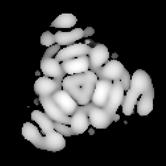
\includegraphics[width=2.7cm]{./flat/HOMO/153-148}
	}
	\subfigure[HOMO - 6]{
		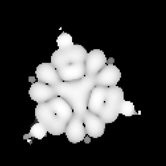
\includegraphics[width=2.7cm]{./B3LYP/HOMO/153-148}
	}
	\subfigure[LUMO + 6]{
		\includegraphics[width=2.7cm]{./B3LYP/LUMO/154-159}
	}
	\subfigure[LUMO + 6]{
		\includegraphics[width=2.7cm]{./flat/LUMO/154-159}
	}
	%%%%%%%%%%%%%%%%%%%%%%%%%%%%%%%%%%%%%%%%%
	\subfigure[HOMO - 12]{
		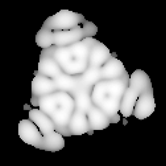
\includegraphics[width=2.7cm]{./flat/HOMO/153-142}
	}
	\subfigure[HOMO - 12]{
		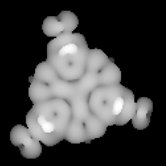
\includegraphics[width=2.7cm]{./B3LYP/HOMO/153-142}
	}
	\subfigure[LUMO + 12]{
		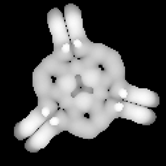
\includegraphics[width=2.7cm]{./B3LYP/LUMO/154-165}
	}
	\subfigure[LUMO + 12]{
		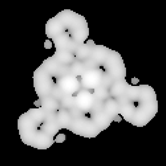
\includegraphics[width=2.7cm]{./flat/LUMO/154-165}
	}
	%%%%%%%%%%%%%%%%%%%%%%%%%%%%%%%%%%%%%%%%%
	\subfigure[HOMO - 18]{
		\includegraphics[width=2.7cm]{./flat/HOMO/153-136}
	}
	\subfigure[HOMO - 18]{
		\includegraphics[width=2.7cm]{./B3LYP/HOMO/153-136}
	}
	\subfigure[LUMO + 18]{
		\includegraphics[width=2.7cm]{./B3LYP/LUMO/154-171}
	}
	\subfigure[LUMO + 18]{
		\includegraphics[width=2.7cm]{./flat/LUMO/154-171}
	}
	%%%%%%%%%%%%%%%%%%%%%%%%%%%%%%%%%%%%%%%%%
	\subfigure[HOMO - 24]{
		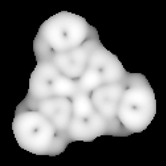
\includegraphics[width=2.7cm]{./flat/HOMO/153-130}
	}
	\subfigure[HOMO - 24]{
		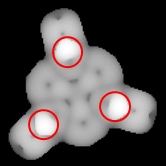
\includegraphics[width=2.7cm]{./B3LYP/HOMO/153-130-mod}
	}
	\subfigure[LUMO + 24]{
		\includegraphics[width=2.7cm]{./B3LYP/LUMO/154-177-mod}
	}
	\subfigure[LUMO + 24]{
		\includegraphics[width=2.7cm]{./flat/LUMO/154-177-mod}
	}
	\caption{EHT calculated molecular orbitals. HOMO and LUMO states together with five neighboring states (shown in the same column). Inner two columns show HOMO \& LUMO states. Outer columns show integration of states as STM image estimation if all states to $E_F$ were contributing equally. Images are \SI{2.5}{\nano \meter} wide}
	
\end{figure}
\vfill